
\begin{enumerate}

\item If the probability of a player winning a game is 0.79, then the probability of his losing the same game is:
\begin{enumerate}    
    \item $1.79$
    \item $0.31$
    \item $0.21	$                                                           
    \item $0.21$
\end{enumerate}

\item From the data $1, 4, 7, 9, 16, 21, 25$, if all the even numbers are removed, then the probability of getting at random a prime number from the remaining is:
	\begin{enumerate}
\item $\frac{2}{5}$
    \item $\frac{1}{5}$
    \item $\frac{1}{7}$
    \item $\frac{2}{7}$
	\end{enumerate}

\item For some data $x_{1}, x_{2}, \dots, x_{n}$ with respective frequencies $f_{1}, f_{2}, \dots, f_{n}$, the value of $\sum_{i}^{n}f_{i} \brak{x_{i} - \overline{x}}$ is equal to:
	\begin{enumerate}    
\item $n \overline{x}$
    \item $1$
    \item $\Sigma f_{i}$
    \item $0$
	\end{enumerate}

\item The middle-most observation of every data arranged in order is called:
	\begin{enumerate}    
\item mode
    \item median
    \item mean
    \item deviation
\end{enumerate}
\newpage
\item Two dice are rolled together. The probability of getting a sum of numbers on the two dice as $2$, $3$, or $5$ is:
	\begin{enumerate}    
\item $\frac{7}{36}$
    \item $\frac{11}{36}$
    \item $\frac{5}{36}$
    \item $\frac{4}{9}$
	\end{enumerate}

item At in a pack of 52 playing cards one card is lost. From the remain cards, a card is drawn at random.
Find the probability that the drawn card is queen of heart, if the lost card is a black card.
\item BINGO is game of chance. The host has $75$ balls numbered $1$ through $75$. Each player has a BINGO ca
rd with some numbers written on it.
The participant cancels the number on the card when called out a number written on the ball selected at rand
om. Whosoever cancels all the numbers on his/her card, says BINGO and wins the game.

\begin{figure}[!ht]
\centering
	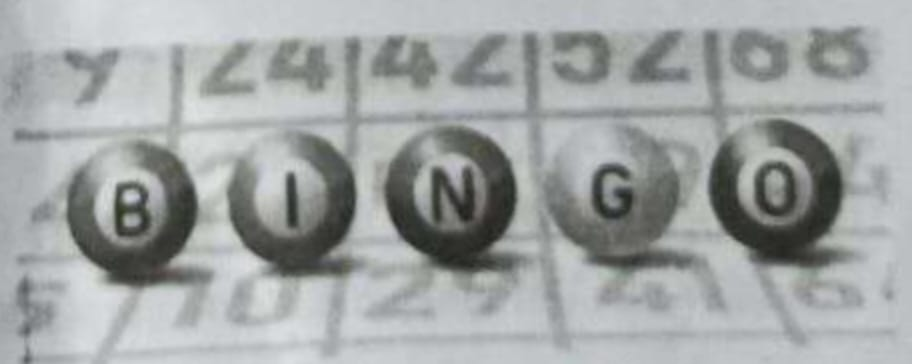
\includegraphics[width=\columnwidth]{figs/p1.jpg}
\label{fig:image 6}
\caption{image 6}
\end{figure}

\text The table given below,shows the data of one game where $48$ ball were used before Tara said "BINGO".
\begin{center}
\begin{tabular}{|c|c|}
\hline
Numbers announced & Number of times \\
\hline
0-15 & 8 \\
\hline
15-30 & 9 \\
\hline
30-45 & 9 \\
\hline
45-60 & 10 \\
\hline
60-75 & 12 \\ 
	\hline
\end{tabular}
\end{center}
 Based on the above information, answer the following:\
\begin{enumerate}
\item Write the median class.\
\item When first ball was picked up,what was the probability of calling out an even umber?\
\item Find median and mode of an the given data.
\end{enumerate}




\end{enumerate}
